\documentclass[9pt, compress, xcolor=table]{beamer}


\usetheme{m}

\usepackage{amsmath,amssymb,amsthm}
\usepackage{latexsym}
\usepackage{booktabs}
\usepackage[scale=2]{ccicons}
\usepackage{minted}
% \usepackage[utf8]{inputenc}
% \usepackage[T2A]{fontenc}
% \usepackage[english, russian]{babel}
%%% For accessing system, OTF and TTF fonts
%%% (would have been loaded by polylossia anyway)
\usepackage{fontspec}
%%% For language switching -- like babel, but for xelatex
\usepackage{polyglossia}
\setmainfont{PT Sans} % вообще шрифты определяются в теме бимера
\setmainlanguage{russian}
\setotherlanguages{english} %% or other languages

\usepackage{graphicx}
\usepackage{xcolor}
\usepackage{tabu} % https://ru.sharelatex.com/learn/Tables
\DeclareGraphicsExtensions{.pdf,.jpg,.png}
\graphicspath{{../images/}{./images/}}

\colorlet{Mycolor1}{green!50!blue!50!}

\usemintedstyle{trac}

\title{Физические принципы микроскопии сверхвысокого разрешения}
\subtitle{осенний семестр, 2018}
\author{ассистент, к.ф.-м.н. Шутова О.А.}
\institute{МГУ им. М.В. Ломоносова, физический факультет}

\begin{document}

\maketitle

\plain{}{Лекция 5. Нелинейная ближнепольная микроскопия}

\begin{frame}{Нелинейная БП микроскопия}

\begin{columns}[c]
\column{6.5cm}

\begin{itemize}
    \item Под нелинейной ближнепольной микроскопией понимают такой вид ближнепольной зондовой микроскопии, когда взаимодействие между электромагнитным полем с веществом образца и зонда носит нелинейный характер. 

\item В первую очередь, это микроскопия на основе генерации второй гармоники.


\item Нелинейная микроскопия развивается в группе профессора Маркуса Б. Рашке, Университет штата Колорадо.

\item А также в работах профессора Анатолия В. Заяца, King's College, London.

\item Использованы материалы диссертации C. Neacsu, защищенной в Берлине в 2008 г.
\end{itemize}
\column{6cm}
\begin{center}
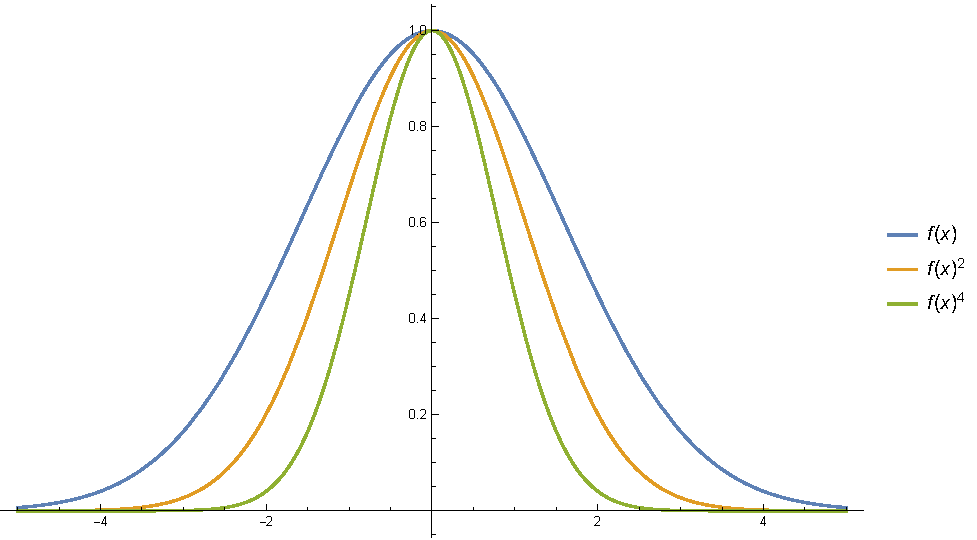
\includegraphics[width=0.9\textwidth]{gauss}
\end{center}
Возведение распределения поля в степень уменьшает величину его пространственной ширины.

\end{columns}
\end{frame}


\begin{frame}{Микроскопия на второй гармонике}
\begin{columns}[c]
\column{6.5cm}
\begin{center}
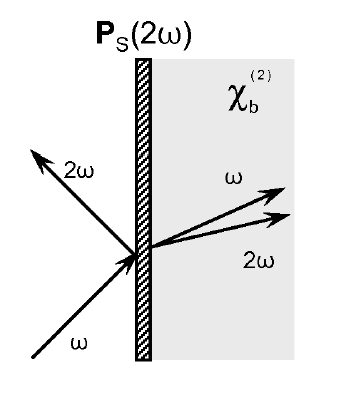
\includegraphics[width=0.7\textwidth]{shg1}

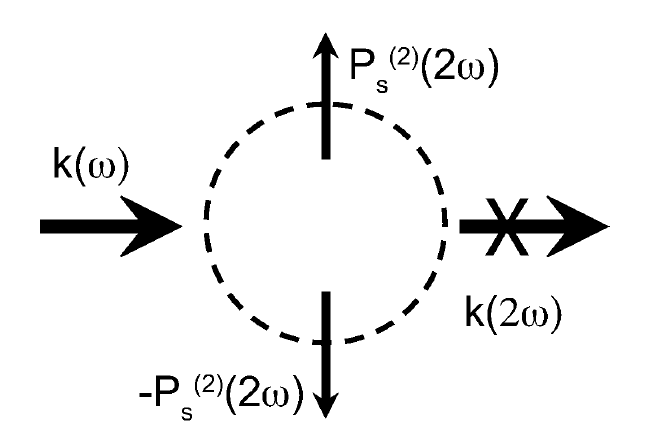
\includegraphics[width=0.65\textwidth]{shg2}
\end{center}
 
\column{6cm}
\vfill Когда среда обладает центральной симметрией (а это 11 из 32 классов симметрии кристаллов) генерация ВГ из объема запрещена. Но это означает, что вторая гармоника исходит от поверхности.
 
\hfill \break В случае сферической частицы (даже в отсутствии ЦС) излучение ВГ вперед будет подавляться деструктивной интерференцией.
 
\hfill \break В ближнем поле генерация ВГ становится более сложным процессом в силу того, что мы уже не можем говорить о направлениях распространения света: преобладают процессы рассеяния. 
\end{columns}
\end{frame}



\begin{frame}{Генерация ВГ от зонда}
\begin{center}
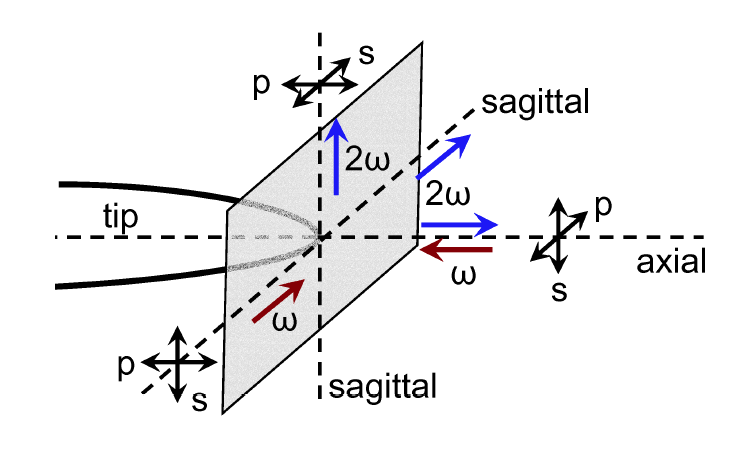
\includegraphics[width=0.6\textwidth]{shg3}
\end{center}

Для ЦС среды генерация ВГ обусловлена вкладом от поверхности, а также электрическим квадрупольным и магнитным дипольным
\begin{multline*}
P^{2\omega}(\vec r) = P^{2\omega}_{surface}(\vec r)+P^{2\omega}_{nonlocal}(\vec r)=\\=\chi^{(2)}_{surface}\otimes \vec E ^{(\omega)}(\vec r)\vec E^{(\omega)}(\vec r)\delta(z)+\chi^{(2)}_{bulk}\otimes \vec E ^{(\omega)}(\vec r)\nabla\vec E ^{(\omega)}(\vec r)
\end{multline*}

Важно учитывать корректировку за счет локального поля как для основной, так и для ВГ

\scriptsize{См. И.Р.Шен <<Принципы нелинейной оптики>>, пар. 25.3. Использование нелинейных оптических эффектов для зондирования поверхности, с.464.}

\end{frame}
\begin{frame}{Генерация ВГ от зонда}
\begin{columns}[c]
\column{6.5cm}

В общем случае у нас остаются ненулевыми следующие вомпоненты 
\begin{equation*}
\chi^{(2)}_{s,zii},\quad\chi^{(2)}_{s,izi}=\chi^{(2)}_{s,iiz},\quad\chi^{(2)}_{s,zzz}
\end{equation*}

Но в силу аксиальной симметричности зонда остаются три компоненты:
\begin{equation*}
\chi^{(2)}_{s,\perp\perp\perp},\quad\chi^{(2)}_{s,\parallel\perp\parallel},\quad\chi^{(2)}_{s,\perp\parallel\parallel}
\end{equation*}

S-пол. это локальный (дипольный) отклик за счет поверхностной $\chi^{(2)}_{surface}$, P- пол. - нелокальный отклик за счет $\chi^{(2)}_{bulk}$ в квадрупольном и магнито-дипольном приближнении
 
\column{6cm}
\begin{center}
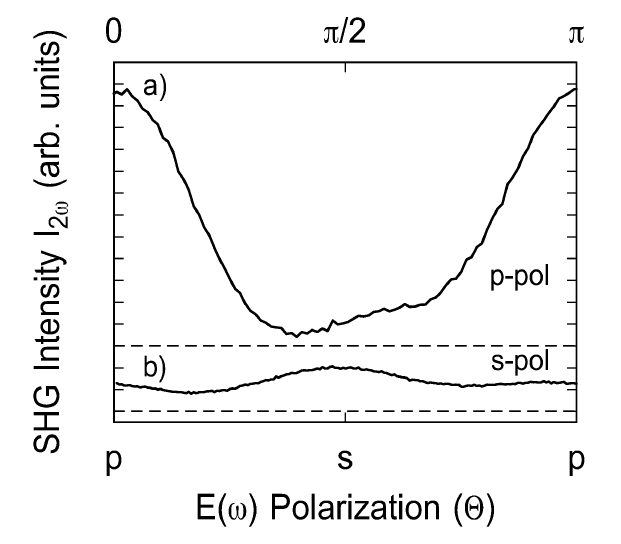
\includegraphics[width=0.9\textwidth]{shg5}
\* $saggital_{in}-saggital_{out}$ наблюдение для разных поляризаций
\end{center}
\end{columns}

\begin{center}
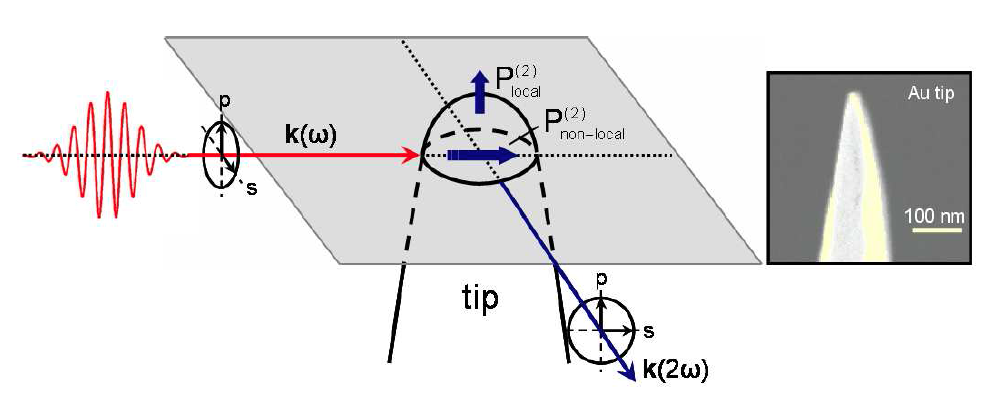
\includegraphics[width=0.6\textwidth]{shg4}
\end{center}

\end{frame}

\begin{frame}{Обобщение эксперимента}

В геометрии \textcolor{blue}{$saggital_{in}-saggital_{out}$} (нет зеркальной симметрии):
\begin{itemize}
\item отклик $p_{in}p_{out}$ исходит от локального дипольного отклика за счет поверхностной квадратичной нелинейности
\item отклик $p_{in}s_{out}$ и $s_{in}s_{out}$ происходят от нелокального квадрупольного и магнитного дипольного компонента квадратичной нелинейности
\item отклик $s_{in}p_{out}$ отсутсвует
\end{itemize}

Таким образом, в этой случае играют роль все поляризации, мы можем получать сигнал обладающий уникальными для зондовой геометрии свойствами.

В геометрии  \textcolor{red!50!black}{$saggital_{in}-axial_{out}$} (в одной плоскости лежат $\vec k (\omega)$, $\vec k (2\omega)$ и ось зонда, подключается зеркальная симметрия относительно любой плоскости, рассекающей зонд вдоль его оси):
\begin{itemize}
\item отсутствует отклик на ВГ в направлении вдоль зонда
\item отсутствует отклик для S-пол. на ВГ в обоих случаях 

\end{itemize}
\end{frame}
 
\begin{frame}{Разделение сигналов ближнего и дальнего поля}

Как и в линейной БП микроскопии разделение ближнепольного сигнала (несмотря на то, что он на частоте ВГ) и дальнепольного является нетривиальной задачей. И так же используется свойство ближнего поля зависеть от расстояния на масштабах много меньше длины волны (дальнее поле на таких масштабах от расстояния не зависит). 

Дрожание зонда равно кривизне его кончика, т.е. приблизительно 15 нм.

\begin{center}
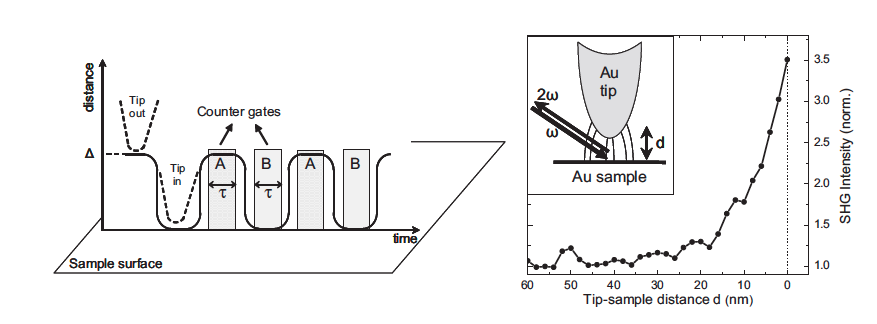
\includegraphics[width=\textwidth]{shg18}
\end{center}

Сигнал отклика равен разности сигналов в положении \emph{ tip in} и \it{tip out}.

\end{frame}

\begin{frame}{Островки алюминия на стеклянной подложке}

\begin{center}
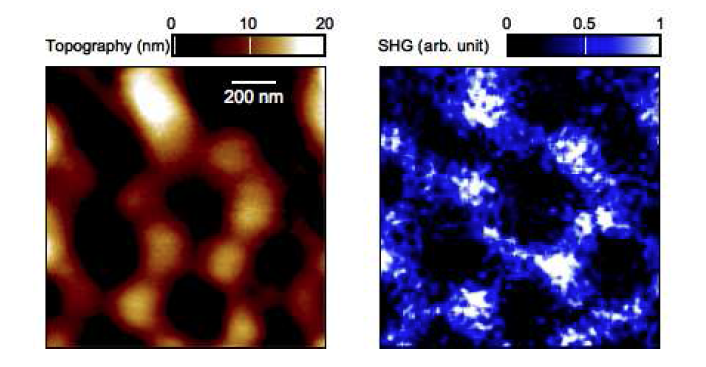
\includegraphics[width=0.7\textwidth]{shg7}
\newline {\scriptsize Падающее поле p поляризовано, ВГ наблюдается без разрешения поляризации}
\end{center}

В случае, когда квадратичная восприимчивость образца много меньше, чем зонда, можно считать, что процесс генерации ВГ происходит только в зонде (как в случае стеклянной подложки). 
В общем случае:

\begin{equation*}
I(2\omega)\propto |\sum_i\chi^{(2)}_{i}\alpha^{eff}_i(\omega)^2+\chi^{(2)}_{t}\alpha^{eff}_t(\omega)^2|^2 E^4(\omega)
\end{equation*}
причем эффективные поляризуемости зависят, каждая от поляризуемости и зонда, и образца.
\end{frame}

\begin{frame}{Аналогичный эксперимент для частичек золота}
\begin{columns}
\column{7cm}
\begin{center}
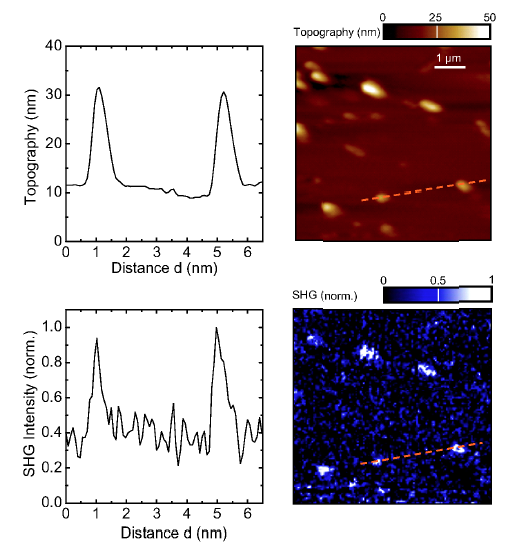
\includegraphics[width=\textwidth]{shg10}
\end{center}
\column{5cm}
Усиление сигнала ВГ над частичками золота достигает двух раз. Некоторые объекты, видимые на топографии, отсутствуют в сигнале ВГ. Следует предположить, что это пылинки или др. дефекты.

Усиление для золота примерно в два раза лучше, чем для алюминия.
\end{columns}
\end{frame}
\plain{}{Исследование сегнетоэлектрических доменов с помощью ближнепольной микроскопии на ВГ}
\begin{frame}{Сегнетоэлектрики}
\begin{columns}
\column{6.5cm}
\begin{center}
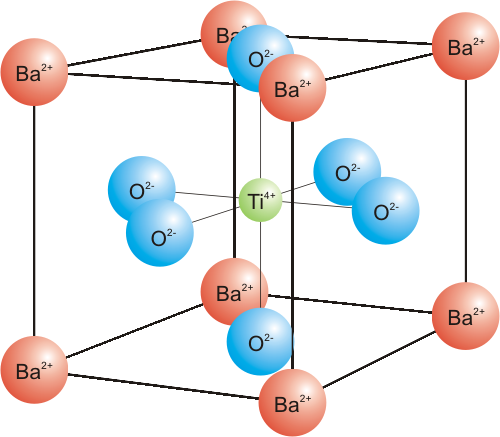
\includegraphics[width=0.7\textwidth]{shg27}
\end{center}
\column{6.5cm}
\begin{center}
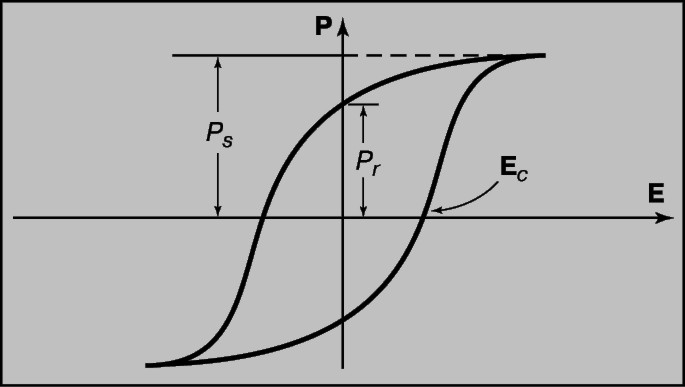
\includegraphics[width=0.8\textwidth]{shg28}
\end{center}

\end{columns}

Самый известный сегнетоэлектрик - титанат бария. При температуре Кюри атом титана скачком смещается из центра на небольшую величину, симметрия переходит из кубической в тетрагональную. Центральному катиону становится энергетически более выгодно сблизиться с одним из анионов, чем быть на равных расстояниях со всеми.  

Исследование сегнетоэлектрических доменов - важное направление в технологии создания оперативной твердотельной памяти (Ferroelectric RAM, FeRAM).

\end{frame}

\begin{frame}{Доменная стенка}
\begin{center}
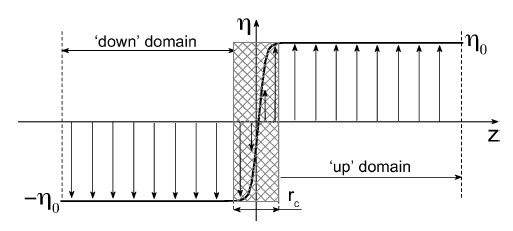
\includegraphics[width=0.8\textwidth]{shg12}
\end{center}

\begin{equation*}
\eta=\pm \sqrt{-\frac{A}{B}}\text{th}\frac{xz}{r_c},\quad \text{где}\quad r_c = \left(\frac{\delta}{A}\right)^{1/2}
\end{equation*}


Эта величина может быть различной для одного и того же материала в разных условиях, варьируется от единиц до десятков ангстрем. В отличие от ферромагнитных доменных стенок, которые состоят из сотен кристаллических ячеек.

\end{frame}

\begin{frame}{Некоторые понятия}

\begin{itemize}
\item \textcolor{red!50!black}{Мультиферроики} -  (или сегнетомагнетиками в советской литературе) называют материалы, в которых сосуществуют одновременно два и более типов «ферро» упорядочения.

\item \textcolor{red!50!black}{Перовскиты} - вещества в основе строения которых лежит кубическая решетка, как у титаната бария с актионно-анионной группой.

\item \textcolor{red!50!black}{Манганиты} - вещества на основе марганца $A_x Mn O_3$, могут иметь решетку типа первоскитов, а могут иметь гексагональную решетку, A -редкоземельный металл, лантан, скандий, иттрий и лантаноиды (57-71).

\item \textcolor{red!50!black}{КМС (колоссальное магнетосопротивление)} -  квантовомеханический эффект заключающийся в сильной зависимости электрического сопротивления материала от величины внешнего магнитного поля. Наблюдается в манганитах.

\item \textcolor{red!50!black}{$Y Mn O_3$} - недавно было обнаружено его свойство быть мультиферроиком, герой нижеследующего изложения.

\end{itemize}

Мультиферроики играют важную роль в разработке энергонезависимой (non volatile) памяти.

\end{frame}

\begin{frame}{Структура}
$Y Mn O_3$ имеет гексагональную структуру
\begin{columns}
\column{10cm}
\begin{center}
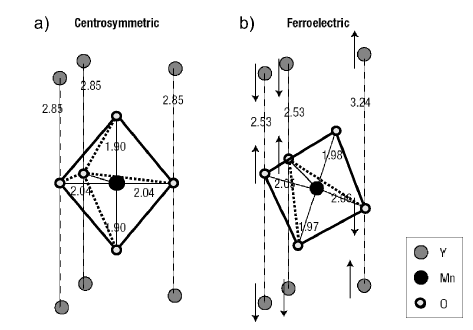
\includegraphics[width=0.8\textwidth]{shg11}
\end{center}
\column{2.5cm}
\centering
\textcolor{blue!50!black}{Неисчезающие $\chi^{(2)}$ в классе $C_{6v}$}:


$\chi^{(2)}_{xzx}=\chi^{(2)}_{xzx}$

$\chi^{(2)}_{xxz}=\chi^{(2)}_{yyz}$

$\chi^{(2)}_{xxz}=\chi^{(2)}_{zyy}$

$\chi^{(2)}_{zzz}$

\end{columns}
Из класса симметрии $6/mmm$ (или $D_{6h}$, гексагональная группа, 24-й порядок) переходит $6mm$ (или $C_{6v}$, гексагональная группа, 12-й порядок, теряет центральную симметрию), $T_c=913^{\circ}$

\end{frame}
\begin{frame}{ВГ от $Y Mn O_3$}

\begin{columns}
\column{6.5cm}
\begin{center}
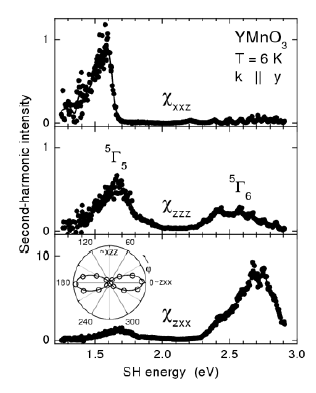
\includegraphics[width=0.8\textwidth]{shg13}

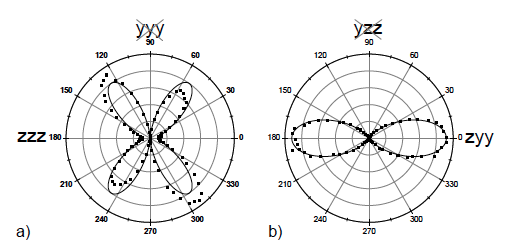
\includegraphics[width=0.7\textwidth]{shg15}
\end{center}
\column{6.5cm}
\begin{center}
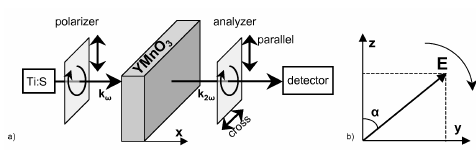
\includegraphics[width=0.9\textwidth]{shg14}
\begin{equation*}
P_x^{(2)}(2\omega) = 2\epsilon_0\chi_{xxz}E^x(\omega)E^z(\omega)
\end{equation*}
\begin{equation*}
P_y^{(2)}(2\omega) = 2\epsilon_0\chi_{xxz}E^y(\omega)E^z(\omega)
\end{equation*}
\begin{equation*}
P_x^{(2)}(2\omega) = 2\epsilon_0\chi_{xxz}E^x(\omega)E^z(\omega)
\end{equation*}

Для величины сигнала:
\begin{equation*}
I_{||}^{SH} \propto \chi_{zzz}^{(2)}E^4 \cos^6 \alpha +\chi_{zyy}^{(2)}E^4 \sin^4 \alpha
\end{equation*}
\begin{equation*}
I_{cross}^{SH} \propto \chi_{zyy}^{(2)}E^4 \cos^6 \alpha
\end{equation*}
\end{center}

\end{columns}

\end{frame}

\begin{frame}{Усиление сигнала ВГ}

Общее изучение характера усиления ближнепольного сигнала второй гармоники 

\begin{center}
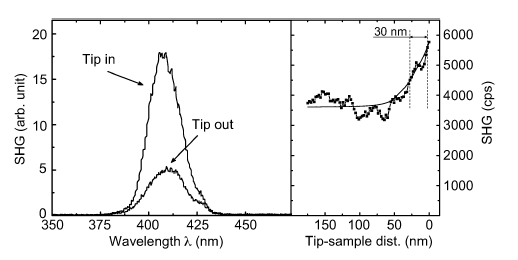
\includegraphics[width=0.8\textwidth]{shg16}

\end{center}

Для p-поляризованного падающего поля под углом $70 ^{(o)}$ (в таком случае $E_x = E \sin 70^{o} = 0.94 E$, а $E_y = E \cos 70 ^{o} = 0.34 E$).

\end{frame}

\begin{frame}{Разрешение отклика по поляризации}

Как отделить сигнал второй гармоники, исходящий от сегнетоэлектрических доменов, от второй гармоники, генерируемой зондом?

Необходимо, апеллируя к приведенным выше исследованиям зонда, выбрать область, где сигнал от зонда минимален ($p_{in} - s_{out}$). Здесь как раз будет играть роль $\chi_{zxx}^{(2)}$ (поле поляризовано вдоль оси $z$ образца).

\begin{center}
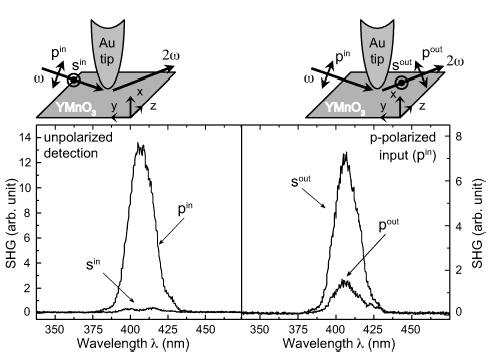
\includegraphics[width=0.7\textwidth]{shg17}

\end{center}

\end{frame}

\begin{frame}{Визуализация сегнетоэлектрических доменов}

\begin{center}
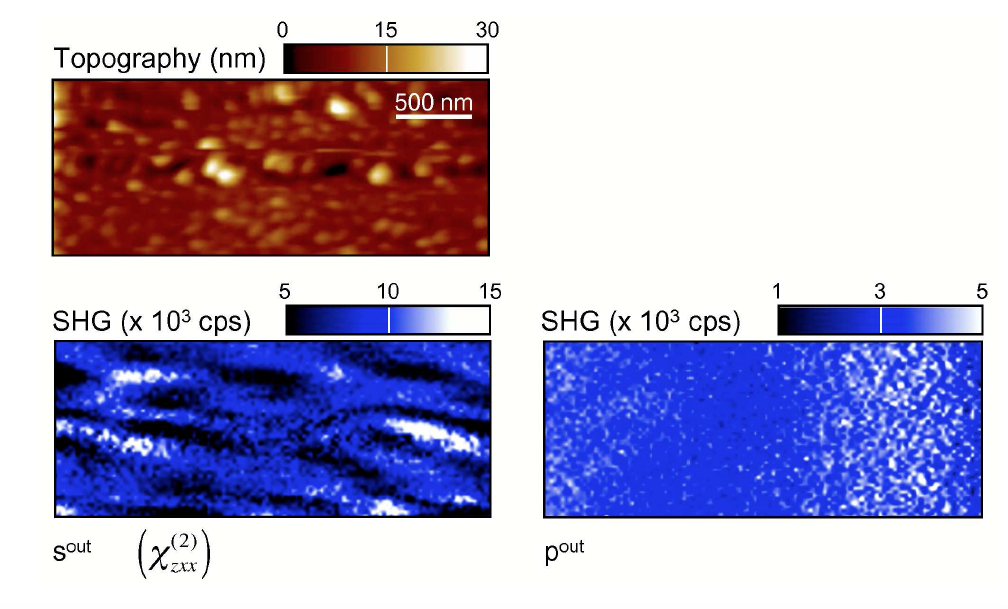
\includegraphics[width=0.8\textwidth]{shg19}

\end{center}

Слева мы видим картину, интерференционного сложения дальнепольного и ближнепольного сигнала второй гармоники, условия для которой меняются при переходе через доменную стенку. Справа мы находимся в области доминирования сигнала ВГ от зонда.


\end{frame}

\begin{frame}{Визуализация сегнетоэлектрических доменов}

\begin{center}
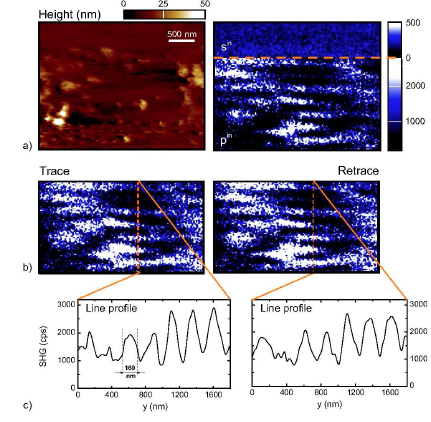
\includegraphics[width=0.8\textwidth]{shg20}

\end{center}

\end{frame}
\begin{frame}{Рассеяние без БП контраста}

\begin{center}
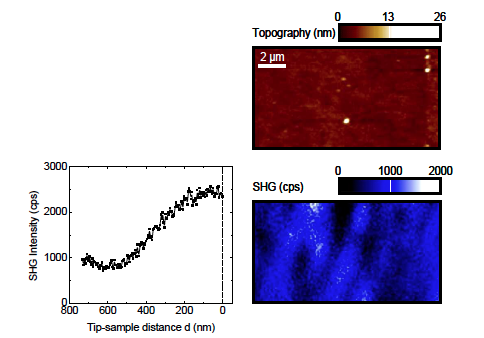
\includegraphics[width=0.8\textwidth]{shg22}

\end{center}

Чувствительность ближнего поля к форме, размеру, шероховатости его поверхности, приводит к тому, что далеко не каждый экземпляр зонда, дает хороший ближнепольный сигнал.


\end{frame}

\begin{frame}{Разрешающая способность}

\begin{columns}
\column{6.5cm}
\begin{center}
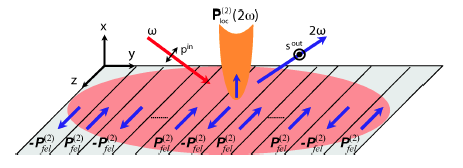
\includegraphics[width=0.8\textwidth]{shg23}

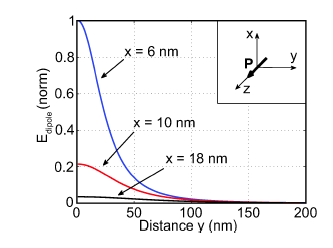
\includegraphics[width=0.6\textwidth]{shg25}

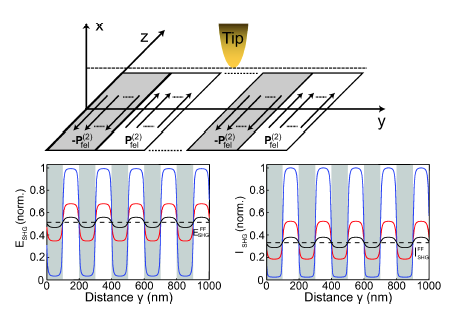
\includegraphics[width=0.7\textwidth]{shg24}
\end{center}

\column{6cm}

В фокусе (2.5 $\mu$м) много доменов участвуют в общей поляризации, связанной с СЭ
\begin{equation*}
\vec P^{(2)}_{FF}(2\omega) = \sum_{i=1}^{N_1}(\vec P^{(2)}_{fel})_i(2\omega)+ \sum_{i=1}^{N_2}(\vec P^{(2)}_{fel})_i(2\omega)
\end{equation*}
БП ВГ локализуется исключительно в области под зондом
\begin{equation*}
\vec P^{(2)}_{loc}(2\omega) \propto L(2\omega)L(\omega)L(\omega)a P^{(2)}_{fel})_i(2\omega)
\end{equation*}
Интерференционная картина:
\begin{equation*}
I(2\omega) \propto \left|P^{(2)}_{FF})_i(2\omega) \pm \vec P^{(2)}_{loc}(2\omega)\right|^2
\end{equation*}

{\scriptsize 10 антипараллельных доменов из 20 диполей каждый, расстояние между диполями 5 нм, в зависимости от расстояния от зонда 6 нм (синий), 10 нм (красный), 18 нм (черный).}

\end{columns}
\end{frame}

\begin{frame}{Эксперимент группы М. Рашке 2018 г.: наклон зонда}

\begin{center}
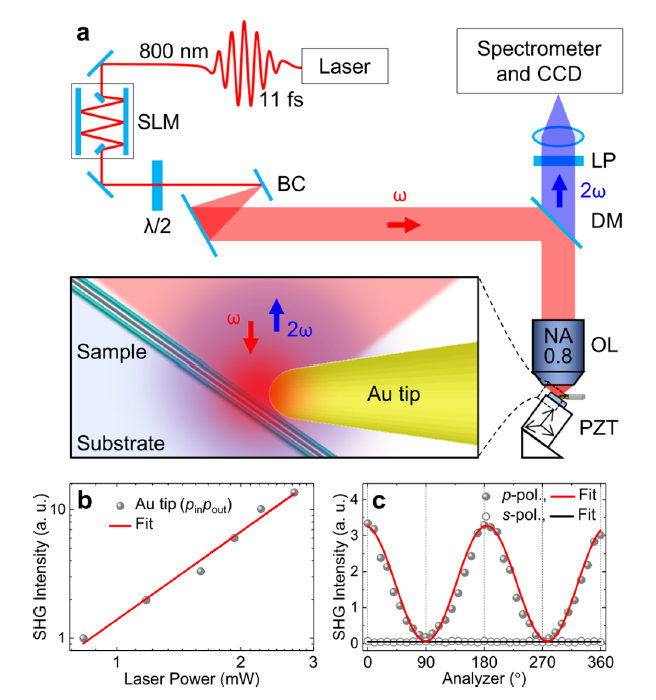
\includegraphics[width=0.8\textwidth]{shg31}

\end{center}




\end{frame}

\begin{frame}{Эксперимент группы М. Рашке 2018 г.: наклон зонда}
Нанокристаллографическая визуализация слоя сульфида молибдена на кремниевой подложке ($MoS_2$) с группой симметрии $\bar{6}m2$

\begin{center}
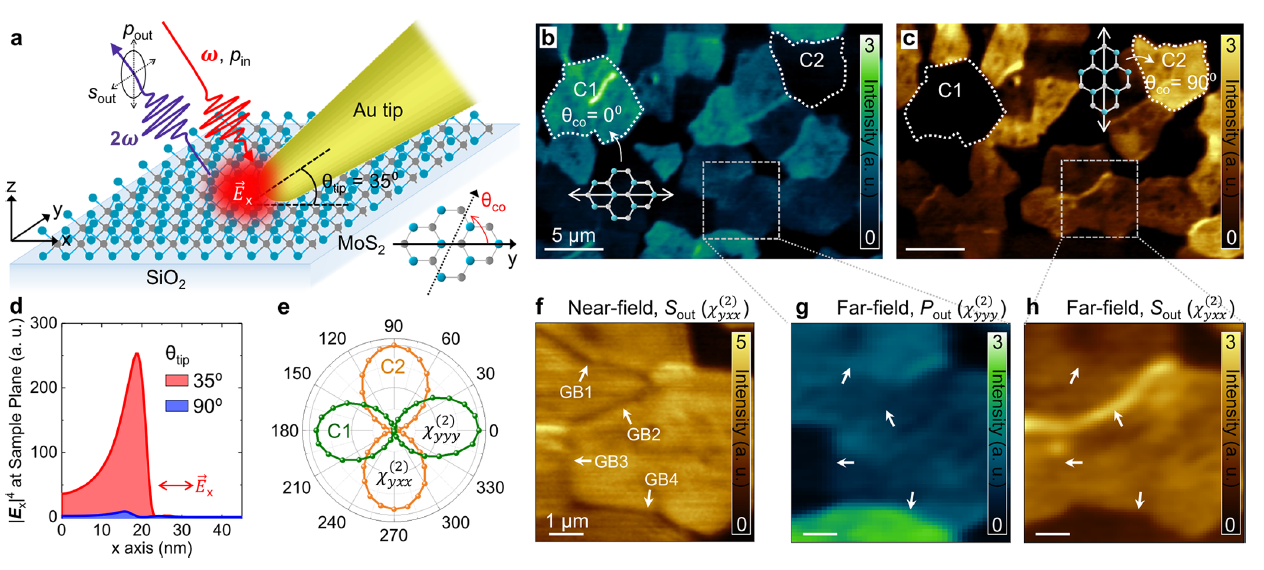
\includegraphics[width=0.8\textwidth]{shg32}


\small{Nano Letters. 2018. Polarization Control with Plasmonic Antenna Tips: A Universal Approach to OPtical Nanocrystallography and Vector-Field Imaging.}
\end{center}

Кристаллы, ориентированные под углом $\theta = 0^\circ$, параллельны падающему полю и поэтому видны в схеме $p_{in}p_{out}$ 

Кристаллы, ориентированные под углом $\theta = 90^\circ$, видны в схеме $p_{in}s_{out}$

\end{frame}

\begin{frame}{Эксперимент группы М. Рашке 2018 г.: наклон зонда}

\begin{center}
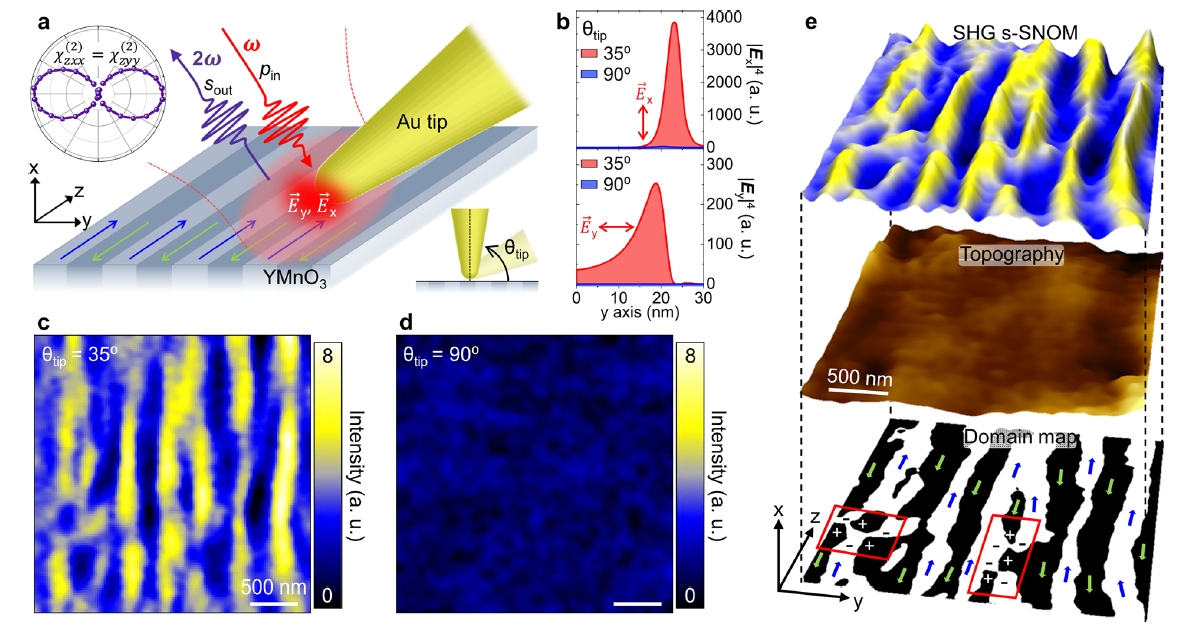
\includegraphics[width=0.8\textwidth]{shg33}

\end{center}

Эксперимент, описанный выше (по визуализации сегнетоэлектрических доменов в манганите иттрия) в схеме с наклонным зондом.

\end{frame}


\end{document}
